\documentclass[a4paper,12pt]{extarticle}
\usepackage[utf8x]{inputenc}
\usepackage[T1,T2A]{fontenc}
\usepackage[russian]{babel}
\usepackage{hyperref}
\usepackage{indentfirst}
\usepackage{listings}
\usepackage{color}
\usepackage{here}
\usepackage{array}
\usepackage{multirow}
\usepackage{graphicx}

\usepackage{caption}
\renewcommand{\lstlistingname}{Программа} % заголовок листингов кода

\bibliographystyle{ugost2008ls}

\usepackage{listings}
\lstset{ %
extendedchars=\true,
keepspaces=true,
language=C,						% choose the language of the code
basicstyle=\footnotesize,		% the size of the fonts that are used for the code
numbers=left,					% where to put the line-numbers
numberstyle=\footnotesize,		% the size of the fonts that are used for the line-numbers
stepnumber=1,					% the step between two line-numbers. If it is 1 each line will be numbered
numbersep=5pt,					% how far the line-numbers are from the code
backgroundcolor=\color{white},	% choose the background color. You must add \usepackage{color}
showspaces=false				% show spaces adding particular underscores
showstringspaces=false,			% underline spaces within strings
showtabs=false,					% show tabs within strings adding particular underscores
frame=single,           		% adds a frame around the code
tabsize=2,						% sets default tabsize to 2 spaces
captionpos=t,					% sets the caption-position to top
breaklines=true,				% sets automatic line breaking
breakatwhitespace=false,		% sets if automatic breaks should only happen at whitespace
escapeinside={\%*}{*)},			% if you want to add a comment within your code
postbreak=\raisebox{0ex}[0ex][0ex]{\ensuremath{\color{red}\hookrightarrow\space}},
texcl=true,
inputpath=listings,                     % директория с листингами
}

\usepackage[left=2cm,right=2cm,
top=2cm,bottom=2cm,bindingoffset=0cm]{geometry}

%% Нумерация картинок по секциям
\usepackage{chngcntr}
\counterwithin{figure}{section}
\counterwithin{table}{section}

%%Точки нумерации заголовков
\usepackage{titlesec}
\titlelabel{\thetitle.\quad}
\usepackage[dotinlabels]{titletoc}

%% Оформления подписи рисунка
\addto\captionsrussian{\renewcommand{\figurename}{Рисунок}}
\captionsetup[figure]{labelsep = period}

%% Подпись таблицы
\DeclareCaptionFormat{hfillstart}{\hfill#1#2#3\par}
\captionsetup[table]{format=hfillstart,labelsep=newline,justification=centering,skip=-10pt,textfont=bf}

%% Путь к каталогу с рисунками
\graphicspath{{fig/}}

%% Внесение titlepage в учёт счётчика страниц
\makeatletter
\renewenvironment{titlepage} {
 \thispagestyle{empty}
}
\makeatother


\begin{document}	% начало документа

% Титульная страница
\begin{titlepage}	% начало титульной страницы

	\begin{center}		% выравнивание по центру

		\large Санкт-Петербургский Политехнический Университет Петра Великого\\
		\large Институт компьютерных наук и технологий \\
		\large Кафедра компьютерных систем и программных технологий\\[6cm]
		% название института, затем отступ 6см
		
		\huge Базы данных\\[0.5cm] % название работы, затем отступ 0,5см
		\large Отчет по лабораторной работе №1\\[0.1cm]
		\large Разработка структуры БД\\[5cm]

	\end{center}


	\begin{flushright} % выравнивание по правому краю
		\begin{minipage}{0.25\textwidth} % врезка в половину ширины текста
			\begin{flushleft} % выровнять её содержимое по левому краю

				\large\textbf{Работу выполнил:}\\
				\large Графов Д.И.\\
				\large {Группа:} 33531/2\\
				
				\large \textbf{Преподаватель:}\\
				\large Мяснов А.В.

			\end{flushleft}
		\end{minipage}
	\end{flushright}
	
	\vfill % заполнить всё доступное ниже пространство

	\begin{center}
	\large Санкт-Петербург\\
	\large \the\year % вывести дату
	\end{center} % закончить выравнивание по центру

\thispagestyle{empty} % не нумеровать страницу
\end{titlepage} % конец титульной страницы

\vfill % заполнить всё доступное ниже пространство


% Содержание
% Содержание
\renewcommand\contentsname{\centerline{Содержание}}
\tableofcontents
\newpage




\section{Цель работы}
Познакомить студентов с возможностями реализации более сложной обработки данных на стороне сервера с помощью хранимых процедур.

\section{Программа работы}
\begin{enumerate}
	\item Создание двух триггеров: один триггер для автоматического заполнения ключевого поля, второй триггер для контроля целостности данных в подчиненной таблице при удалении/изменении записей в главной таблице.
	\item Создание триггера в соответствии с индивидуальным заданием, полученным у преподавателя.
	\item Создание триггера в соответствии с индивидуальным заданием, вызывающего хранимую процедуру.
	\item Выкладывание скрипта с созданными сущностями в GitLab.
	\item Демонстрация результатов преподавателю.
\end{enumerate}

\section{Ход работы}
\subsection{Триггер для автоматического заполнения ключевого поля}
Для тестирования создадим таблицу test\_table и последовательность test\_table\_seq, из которой будут браться значения primary key.
\begin{lstlisting}[caption=Создание таблицы и последовательности для неё, language=SQL]
create sequence if not exists test_table_seq as int start with 1;

create table if not exists test_table
(
	id    int primary key not null,
	value int
);
\end{lstlisting}

Теперь создадим триггер и процедуру для него. Триггер будет срабатывать перед добавлением новых значений в таблицу. Он будет брать параметр new и добавлять в него следующее значение последовательности.

\begin{lstlisting}[caption=Создание триггера и процедуры для него, language=SQL]
create or replace function test_id_correction() returns trigger as
$$
begin
	new.id = nextval('test_table_seq');
	return new;
end;
$$ language plpgsql;

create trigger auto_upd
	before insert
	on test_table
	for each row
execute procedure test_id_correction();

insert into test_table (value)
values  (1),
		(2),
		(3),
		(4);

select *
from test_table;
\end{lstlisting}

Протестируем созданный триггер. Добавим последовательность значений в таблицу и убедимся, что primary key расставлены верно.

\begin{lstlisting}[caption=Добавление новых значений в таблицу, language=SQL]
insert into test_table (value)
values  (1),
		(2),
		(3),
		(4);

select *
from test_table;
\end{lstlisting}

\begin{figure}[H]
	\begin{center}
		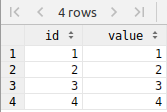
\includegraphics[scale=0.7]{common_1}
		\caption{Результат выполнения запроса} 
		\label{pic:1} % название для ссылок внутри кода
	\end{center}
\end{figure}
Как видим, первичные ключи автоматически добавились в кортежи.

\subsection{Триггер для контроля целостности данных в подчинённой таблице}

Создадим две таблицы: test\_table\_master (далее: master) и test\_table\_slave (далее: slave), при этом поле master\_id таблицы slave ссылается на поле id из таблицы master.

\begin{lstlisting}[caption=Создание тестовых таблиц, language=SQL]
create table if not exists test_table_master
(
	id    int primary key not null,
	value int
);

create table if not exists test_table_slave
(
	id        int primary key not null,
	master_id int references test_table_master (id),
	name      text
);
\end{lstlisting}

Теперь нужно создать два триггера (before update(delete) и after update) и две процедуры для них.

Алгоритм для обновления:
перед тем, как обновить данные в таблице master, в ней же создаётся запись с id = -1. Все записи в таблице slave, которые зависят от изменяемого master.id, меняют свои master\_id на -1. Затем в таблице master происходит обновление, после чего все записи slave, у которых в поле master\_id стоит -1, меняют его на обновлённое значение.

При удалении же вызывается триггер только before delete, в котором удаляются зависимые значения из таблицы slave.

\begin{lstlisting}[caption=Код триггеров и процедур, language=SQL]
create or replace function slave_update_before_func()
	returns trigger as
$$
begin
	if (tg_op = 'DELETE') then
		delete from test_table_slave where master_id = old.id;
		return old;
	end if;
	raise notice 'start updating';
	--create fake record in master
	insert into test_table_master values (-1, 0);
	--redirect slave to fake record
	update test_table_slave set master_id = -1 where master_id = old.id;
	raise notice 'slave redirected';
	return new;
end;
$$ language plpgsql;

create or replace function slave_update_after_func()
	returns trigger as
$$
begin
	--redirect slave to new record
	update test_table_slave set master_id = new.id where master_id = -1;
	raise notice 'slave redirect back';
	--delete fake record
	delete from test_table_master where id = -1;
	return new;
end;
$$ language plpgsql;

create trigger slave_update_before
	before update or delete
	on test_table_master
	for each row
execute procedure slave_update_before_func();

create trigger slave_update_after
	after update
	on test_table_master
	for each row
execute procedure slave_update_after_func();
\end{lstlisting}

Протестируем триггеры. Сначала посмотрим, что находится в таблице master и slave.

\begin{figure}[!htb]
	\minipage{0.5\textwidth}
	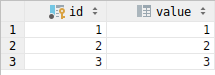
\includegraphics[width=\linewidth]{master_before}
	\caption{Таблица master}\label{fig:master}
	\endminipage\hfill
	\minipage{0.5\textwidth}
	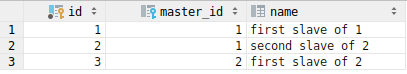
\includegraphics[width=\linewidth]{slave_before}
	\caption{Таблица slave}\label{fig:slave}
	\endminipage\hfill
\end{figure}

Выполним следующие запросы.

\begin{lstlisting}[caption=Обновление и удаление данных из master, language=SQL]
update test_table_master
set id = 4
where id = 2;

delete
from test_table_master
where id = 1;
\end{lstlisting}

\begin{figure}[!htb]
	\minipage{0.5\textwidth}
	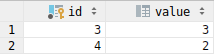
\includegraphics[width=\linewidth]{master_after}
	\caption{Таблица master}\label{fig:master_after}
	\endminipage\hfill
	\minipage{0.5\textwidth}
	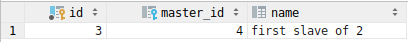
\includegraphics[width=\linewidth]{slave_after}
	\caption{Таблица slave}\label{fig:slave_after}
	\endminipage\hfill
\end{figure}

Как видим, данные были успешно удалены и изменены как в master, так и в slave

\subsection{Триггер, автоматически рассчитывающий среднюю цену товаров (напитков и еды) при добавлении новых поставок}

\lstinputlisting[
language=SQL,
caption={sp1.sql},
]{../../src/ind1.sql}

Создадим две процедуры, расчитывающие и возвращающие в качечестве атрибута new.price\_per\_item среднюю цену из таблицы drinks и таблицы food (строки 1-15).
Далее создадим триггеры, использующие данные процедуры перед вставкой нового кортежа (строки 17 - 27).
Таким образом, про добавлении новой записи в таблицу supplies\_drinks поле average\_price автоматически заполняется средним значением цены из таблицы drinks.
Протестируем работу триггеров (строки 29 - 36).

\begin{figure}[H]
	\begin{center}
		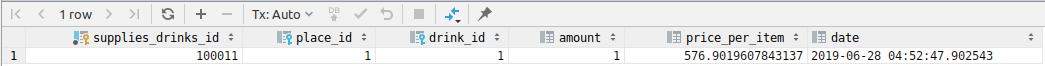
\includegraphics[scale=0.5]{sd}
		\caption{Новый кортеж таблицы supplies\_drinks} 
		\label{pic:sf} % название для ссылок внутри кода
	\end{center}
\end{figure}

\begin{figure}[H]
	\begin{center}
		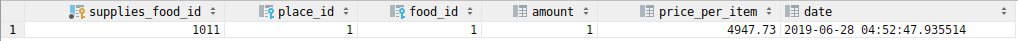
\includegraphics[scale=0.5]{sf}
		\caption{Новый кортеж таблицы supplies\_food} 
		\label{pic:sd} % название для ссылок внутри кода
	\end{center}
\end{figure}

\subsection{Триггер, запрещающий добавлять одни и те же позиции товара с разными стоимостями в один и тот бар}

\lstinputlisting[
language=SQL,
caption={sp1.sql},
]{../../src/ind2.sql}

Добавим новые позиции в таблицу drinks с одинаковыми названиями (строки 1 - 3).
Создадим функцию, которая при равенстве названия и неравенстве стоимости существующей записи и новой в таблице places\_drinks в бросает exception с описанием 'Error! Trying to add new item with different price.' (строки 5 - 28). Создадим триггер, вызывающий процедуру перед добавлением записи а places\_drinks (строки 30 - 34). Попробуем добавить две новые позиции с одинаковым названием и разной стоимостью в бар с place\_id = 1.

\begin{figure}[H]
	\begin{center}
		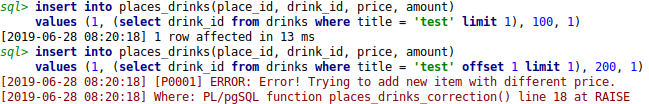
\includegraphics[scale=0.5]{ind2}
		\caption{Попытка добавить одну и ту же позицию товара с разными стоимостями в один бар} 
		\label{pic:ind2} % название для ссылок внутри кода
	\end{center}
\end{figure}

Как мы можем видеть, мы получили ошибку. Ошибка также возникнет, если drink\_id двух записей будут равны.
Но если стоимость этих товаров одинакова, операция пройдёт успешно.

\newpage
\section{Выводы}
В ходе работы были изучены триггеры в PostgreSQL. 

Это очень мощный инструмент
для обработки данных на стороне сервера, расширающий возможности разработчика.

Триггер является указанием, что база данных должна автоматически выполнить за-
данную функцию, всякий раз когда выполнен определённый тип операции. Триггеры мож-
но использовать с таблицами, представлениями и внешними таблицами.

Для обычных и сторонних таблиц можно определять триггеры, которые будут сраба-
тывать до или после любой из команд INSERT, UPDATE или DELETE; либо один раз для
каждой модифицируемой строки, либо один раз для оператора SQL.
Для представлений триггеры могут быть определены для выполнения вместо операций
INSERT, UPDATE и DELETE. Такие триггеры INSTEAD OF вызываются единожды для
каждой строки, которая должна быть изменена в этом представлении. Именно функция
триггера отвечает за то, чтобы произвести необходимые изменения в нижележащих базовых таблицах представления и должным образом возвращать изменённые строки, чтобы
они появлялись в представлении. Триггеры для представлений тоже могут быть определены так, что они будут выполняться единожды для всего оператора SQL, до или после
операций INSERT, UPDATE или DELETE. Однако такие триггеры срабатывают, только
если для представления определён триггер INSTEAD OF. В противном случае все операторы, обращающиеся к представлению, должны быть переписаны в виде операторов,
обращающихся к нижележащим базовым таблицам, и тогда будут срабатывать триггеры,
установленные для этих таблиц.

Триггерная функция должна быть создана до триггера. Она должна быть объявлена без аргументов и возвращать тип trigger. (Триггерная функция получает данные на
вход посредством специально переданной структуры TriggerData, а не в форме обычных
аргументов.)

После создания триггерной функции создаётся триггер с помощью CREATE TRIGGER.
Одна и та же триггерная функция может быть использована для нескольких триггеров.

В результате работы были созданы триггеры для автоматического заполнения ключевого поля в таблице и сохранения целостности данных в зависимой таблице при изменении
или удалении данных в главной таблице. Также были созданы триггеры по заданию преподавателя: для подсчёта средней стоимости позиции и для запрета добавления новой позиции с существующим названием и новой стоимостью.
\end{document}
